\documentclass[sigconf]{webmedia}

\usepackage[brazil]{babel}
\usepackage{booktabs}

\usepackage{adjustbox}
\usepackage{listings}
\usepackage{xurl}
\hypersetup{urlcolor=black}

\settopmatter{printacmref=false, printfolios=true}
\proceedingsDetails[Teoria dos Grafos, 2026]{Trabalho Acadêmico de Teoria dos Grafos}{2026}{UFBA}
\acmBooktitle{Trabalho Acadêmico de Teoria dos Grafos}
\acmDOI{}
\ISSN{}
\copyrightyear{2026}
\makeatletter
\def\@copyrightpermission{In: \proceedingsDetails@name\ (\proceedingsDetails@shortname). UFBA. Salvador, 2026.}
\def\@copyrightowner{Instituto de Computação da UFBA}
\makeatother

\lstset{
  basicstyle=\ttfamily\scriptsize,
  columns=fullflexible,
  keepspaces=true,
  breaklines=true,
  frame=single,
  showstringspaces=false,
  literate={á}{{\'a}}1 {ã}{{\~a}}1 {ç}{{\c{c}}}1 {é}{{\'e}}1 {ê}{{\^e}}1 {í}{{\'i}}1 {ó}{{\'o}}1 {õ}{{\~o}}1 {ú}{{\'u}}1
}


\begin{document}

\title{Análise e tratamento de Grafos}
\subtitle{Aplicação sobre a rede de interação face a face do jogo \textit{The Resistance} (SNAP)}

\author{Nadson de Santana Sousa}
\affiliation{%
  \department{Matrícula: 224215945}
  \institution{Instituto de Computação da UFBA}
  \city{Salvador}
  \state{Bahia}
  \country{Brasil}
}

\renewcommand{\shortauthors}{Sousa}

\begin{abstract}
Este trabalho apresenta uma análise estrutural do grafo \textit{comm-f2f-Resistance}, do repositório SNAP, que registra quem olha para quem, a cada $1/3$ de segundo, durante 62 partidas do jogo de dedução social \textit{The Resistance}. O grafo original é temporal, dirigido e ponderado, com mais de 3,1 milhões de arestas temporais. Aplicamos a conversão para um grafo estático por meio da fração de tempo de atenção entre participantes, um limiar de atenção acima do uniforme, a conversão para grafo não-direcionado e a união das 62 partidas, resultando em um grafo de 451 vértices, 951 arestas e 62 componentes. Calculamos todas as métricas estruturais de forma exata, implementamos os algoritmos clássicos da disciplina e investigamos as propriedades \textit{small-world}, lei de potência e robustez. Os resultados mostram uma rede formada por pequenos grupos densos ($\bar{C}=0{,}75$), sem hubs e sem lei de potência, cuja aparente propriedade \textit{small-world} é inteiramente explicada pela partição em partidas.
\end{abstract}

\keywords{redes de interação face a face, SNAP, análise estrutural, algoritmos de grafos, small-world, robustez}

\begin{teaserfigure}
  \centering
  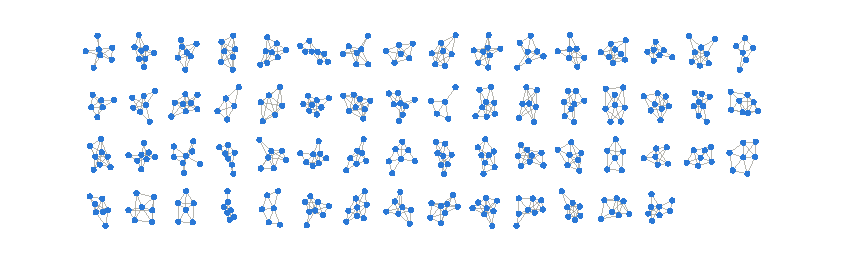
\includegraphics[width=\textwidth]{../figures/grafo_completo.pdf}
  \caption{Grafo completo tratado: 451 vértices (participantes) organizados nas 62 componentes (partidas).}
  \label{fig:teaser}
\end{teaserfigure}

\maketitle

\section{Introdução}
A teoria dos grafos fornece uma linguagem comum para modelar fenômenos muito distintos, como redes sociais, redes de transporte e sistemas biológicos, revelando propriedades estruturais que não aparecem em análises tabulares convencionais. Neste trabalho analisamos uma rede social de escala humana: o olhar entre pessoas que conversam em grupo.

O dataset~\cite{kumar2021,bai2019} contém redes dinâmicas de interação face a face extraídas de vídeos de 62 partidas de \textit{The Resistance}, um jogo em que parte dos jogadores são espiões e tentam enganar os demais. Cada partida tem de 5 a 8 participantes e dura de 16 a 60 minutos. A escolha de analisar este grafo traz um contraste interessante com as redes de grande escala usualmente estudadas: aqui a rede é pequena e fortemente particionada, o que permite calcular todas as métricas de forma exata e discutir quando conceitos como \textit{small-world} e lei de potência fazem (ou não) sentido.

\section{Determinação do Grafo}
A especificação associa a cada estudante um grafo de uma lista numerada $G_1, \dots, G_{129}$ (planilha ANALISANDO-SNAP-DATASET). Dado o número de matrícula $M$, calcula-se a soma $S$ dos seus dígitos e o número $D$ formado pelos seus dois últimos dígitos; o índice do grafo é
\[
  i = (S \times (D + 1)) \bmod 129,
\]
considerando $i = 129$ quando o resultado é 0. A Tabela~\ref{tab:matricula} aplica a regra à matrícula deste trabalho.

\begin{table}[h]
  \caption{Cálculo do grafo a partir da matrícula $M = 224215945$.}
  \label{tab:matricula}
  \begin{tabular}{lr}
    \toprule
    Passo & Valor \\
    \midrule
    Dígitos de $M$ & 2, 2, 4, 2, 1, 5, 9, 4, 5 \\
    Soma dos dígitos $S$ & $2+2+4+2+1+5+9+4+5 = 34$ \\
    Dois últimos dígitos $D$ & 45 \\
    $S \times (D + 1)$ & $34 \times 46 = 1564$ \\
    Divisão por 129 & $1564 = 12 \times 129 + 16$ \\
    $i = 1564 \bmod 129$ & \textbf{16} \\
    \bottomrule
  \end{tabular}
\end{table}

Como $i = 16 \neq 0$, o grafo atribuído é o \textbf{G16 -- comm-f2f-Resistance}, da categoria \textit{Social networks} da coleção SNAP~\cite{snap}: uma rede ponderada, dirigida e temporal com 451 vértices e 3.126.993 arestas temporais. A regra foi conferida com os dois exemplos da especificação: a matrícula 225216327 resulta em $(30 \times 28) \bmod 129 = 66$ e a matrícula 2025000078, em $(24 \times 79) \bmod 129 = 90$.

\section{Códigos}
O código-fonte, o dataset tratado e as instruções de execução estão disponíveis em: \url{https://github.com/NadsonSantana/GrafoG16}. Todos os algoritmos foram implementados em Python sobre uma lista de adjacência própria; a biblioteca NetworkX foi usada apenas como oráculo nos testes automatizados e para o \textit{layout} das visualizações.

\section{Metodologia}

\subsection{Descrição do grafo original}
Cada partida $g$ é distribuída como uma série temporal de matrizes de adjacência binárias: em cada instante $t$ ($1/3$ s), a variável \texttt{Pi\_TO\_Pj} vale 1 se o participante $i$ olha para $j$, e \texttt{Pi\_TO\_LAPTOP} vale 1 se $i$ olha para o próprio laptop. Cada participante olha para exatamente um alvo por instante (grau de saída 1). Há também uma versão ponderada com probabilidades. A Tabela~\ref{tab:dataset} resume o dataset.

\begin{table}[h]
  \caption{Estatísticas do dataset original.}
  \label{tab:dataset}
  \begin{adjustbox}{max width=\columnwidth}
  \begin{tabular}{lr}
    \toprule
    Característica & Valor \\
    \midrule
    Tipo & ponderado, dirigido,\\ & temporal \\
    Partidas (redes) & 62 \\
    Participantes (vértices) & 451 \\
    Instantes registrados & 426.015 \\
    Duração total & 142.005 s \\
    Arestas temporais (part.$\to$part.) & 2.929.953 \\
    Arestas temporais (part.$\to$laptop) & 197.040 \\
    Total de arestas temporais & 3.126.993 \\
    \bottomrule
  \end{tabular}
  \end{adjustbox}
\end{table}

O grafo é modelado como $G = (V, E)$, onde $V$ é o conjunto de participantes e $\{u, v\} \in E$ indica que $u$ e $v$ dedicam atenção visual significativa um ao outro.

\subsection{Tratamento dos dados}
Os seguintes tratamentos foram aplicados, nesta ordem:

\textbf{(1) Grafo temporal $\to$ grafo estático.} Para cada par ordenado $(u, v)$ de uma mesma partida, calculamos a atenção
\[
  f(u, v) = \frac{1}{T}\sum_{t=1}^{T} \mathbb{1}[u \text{ olha para } v \text{ no instante } t],
\]
isto é, a fração do tempo em que $u$ olha para $v$. A dimensão temporal deixa de influenciar a topologia, mas fica preservada no peso.

\textbf{(2) Remoção do alvo laptop e de auto-laços.} O laptop não é um participante, e \texttt{Pi\_TO\_Pi} é sempre 0. Em média, 6,6\% do tempo é dedicado ao laptop.

\textbf{(3) Limiar de atenção.} A união simples de todas as arestas ao longo do tempo gera um grafo praticamente completo: 2.867 dos 2.870 pares ordenados possíveis ocorrem ao menos uma vez. Isso tornaria a análise trivial. Por isso, mantivemos o arco $u \to v$ somente se $f(u, v) \geq 1/N$, onde $N$ é o número de alvos possíveis de $u$ ($N-1$ colegas mais o laptop). O critério tem interpretação direta: $u$ olha para $v$ \emph{mais do que olharia sob atenção uniforme}.

\textbf{(4) Grafo dirigido $\to$ não-direcionado.} A aresta $\{u, v\}$ existe se $u \to v$ ou $v \to u$. Seu peso é a atenção mútua $w = (f(u,v) + f(v,u))/2$, e a distância usada nos algoritmos ponderados é $d = -\ln w > 0$: atenção forte implica distância curta, e a soma de distâncias de um caminho corresponde ao produto das atenções. A versão dirigida foi mantida para o algoritmo de Tarjan.

\textbf{(5) União das 62 partidas.} Cada vértice recebe o identificador \texttt{gXX\_pY} (partida, participante), e as partidas são reunidas em um único grafo. Como participantes de partidas distintas não interagem, cada partida vira uma componente.

O trecho central do tratamento é mostrado a seguir.

\begin{lstlisting}[language=Python]
atencao = dados[:, :, 1:].mean(axis=0)   # f[i, j]
np.fill_diagonal(atencao, 0.0)
limiar = 1.0 / n                          # n alvos possíveis
for i in range(n):
    for j in range(i + 1, n):
        if atencao[i, j] >= limiar or atencao[j, i] >= limiar:
            w = (atencao[i, j] + atencao[j, i]) / 2
            arestas.append((u(i), u(j), w, -math.log(w)))
\end{lstlisting}

A Tabela~\ref{tab:etapas} mostra a evolução do grafo ao longo do tratamento.

\begin{table}[h]
  \caption{Evolução do grafo ao longo dos tratamentos aplicados.}
  \label{tab:etapas}
  \begin{adjustbox}{max width=\columnwidth}
  \begin{tabular}{lrr}
    \toprule
    Etapa & Vértices & Arestas \\
    \midrule
    Grafo temporal bruto (com laptop) & 451 & 3.126.993 \\
    Sem laptop & 451 & 2.929.953 \\
    Estático (pares que ocorrem) & 451 & 2.867 arcos \\
    Após limiar $f \geq 1/N$ & 451 & 1.241 arcos \\
    Não-direcionado (final) & 451 & 951 \\
    \bottomrule
  \end{tabular}
  \end{adjustbox}
\end{table}

\subsection{Visualização do grafo}
A Figura~\ref{fig:teaser} mostra o grafo completo: cada componente corresponde a uma partida. A Figura~\ref{fig:partida0} detalha a partida 0 na versão dirigida, com a espessura do arco proporcional à atenção $f(u,v)$. Nota-se a assimetria: alguns participantes concentram o olhar dos demais.

\begin{figure}[h]
  \centering
  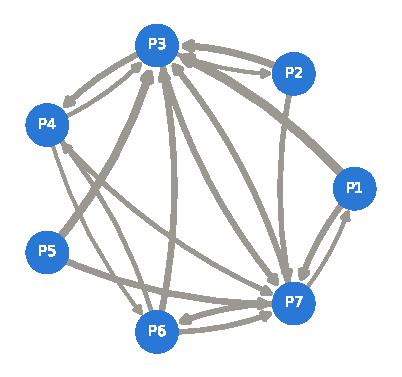
\includegraphics[width=0.6\linewidth]{../figures/partida0.pdf}
  \caption{Partida 0 (7 participantes), versão dirigida. A espessura do arco é proporcional à atenção $f(u,v)$.}
  \label{fig:partida0}
\end{figure}

\subsection{Abordagem para métricas e algoritmos}
\textbf{Cálculo exato.} Com 451 vértices, nenhuma métrica exigiu amostragem: diâmetro, raio e comprimento médio foram obtidos por BFS a partir de \emph{todos} os vértices, e Floyd-Warshall foi executado no grafo inteiro.

\textbf{Grafo desconexo.} Diâmetro, raio e comprimento médio só são definidos dentro de uma componente. Por isso, reportamos esses valores na maior componente conexa (LCC) e também agregados sobre todas as componentes, considerando apenas pares alcançáveis.

\textbf{Pesos reais.} Diferentemente de grafos não-ponderados, aqui os pesos têm significado: Dijkstra, Bellman-Ford, Floyd-Warshall, Prim e Kruskal usam a distância $d = -\ln w$.

\textbf{Implementações iterativas.} DFS e Tarjan usam pilha explícita.

\textbf{Análise temporal.} Cada algoritmo foi executado $n$ vezes, após uma execução de aquecimento. O intervalo de confiança de 95\% da média é $\bar{x} \pm c \cdot s/\sqrt{n}$, com $c = z_{\alpha/2} = 1{,}96$ (Normal) para $n \geq 30$ e $c = t_{\alpha/2,\,n-1}$ (t-Student) para $n < 30$. Usamos $n = 50$ para os algoritmos rápidos, $n = 30$ para Bellman-Ford e $n = 10$ para Floyd-Warshall ($t_{0{,}025;9} = 2{,}262$).

\textbf{Validação.} Uma suíte de 27 testes automatizados compara cada implementação com o NetworkX em grafos aleatórios desconexos e verifica casos de resposta conhecida (caminhos, ciclos, estrelas, ciclos negativos e SCCs).

\section{Resultados}
Os resultados estão divididos em três partes: a análise estrutural obrigatória (Parte I), a aplicação dos algoritmos da disciplina (Parte II) e a análise de propriedades da rede (Parte III).

\subsection{Parte I: Análise Estrutural}
A Tabela~\ref{tab:metricas} apresenta as métricas estruturais do grafo tratado. Todas foram computadas, e de forma exata.

\begin{table}[h]
  \caption{Métricas estruturais do grafo tratado. Todas foram computadas de forma exata (nenhuma por amostragem).}
  \label{tab:metricas}
  \begin{adjustbox}{max width=\columnwidth}
  \begin{tabular}{lrc}
    \toprule
    Métrica & Valor & Computada \\
    \midrule
    Número de vértices & 451 & sim \\
    Número de arestas & 951 & sim \\
    Grau mínimo / máximo & 1 / 7 & sim \\
    Grau médio & 4,2173 & sim \\
    Densidade & $9{,}37 \times 10^{-3}$ & sim \\
    Densidade média intra-partida & 0,6702 & sim \\
    Número de componentes & 62 & sim \\
    Tamanho das componentes & 5 a 8 & sim \\
    Tamanho da LCC & 8 & sim \\
    Diâmetro (LCC / máx. componentes) & 2 / 3 & sim \\
    Raio (LCC / mín. componentes) & 1 / 1 & sim \\
    Comprimento médio (LCC / global) & 1,2857 / 1,3401 & sim \\
    Coef. de clusterização médio & 0,7541 & sim \\
    Número de triângulos & 791 & sim \\
    Visualização & Fig.~\ref{fig:teaser} e \ref{fig:partida0} & sim \\
    \bottomrule
  \end{tabular}
  \end{adjustbox}
\end{table}

\textbf{Densidade e componentes.} A densidade global de $9{,}37 \times 10^{-3}$ sugere um grafo esparso, mas é enganosa: ela é baixa apenas porque não existem arestas entre partidas. Dentro de cada partida, a densidade média é 0,67, ou seja, cada participante presta atenção significativa a dois terços dos colegas. As 62 componentes têm 8 (29 partidas), 7 (23), 6 (8) ou 5 vértices (2) e coincidem exatamente com as partidas: nenhuma partida foi fragmentada pelo limiar, e não há vértices isolados.

\textbf{Distâncias.} O diâmetro máximo entre as componentes é 3, e o da LCC é 2. O comprimento médio dos caminhos é 1,34: a maioria dos pares está ligada diretamente, e os demais por um único intermediário.

\textbf{Clusterização e triângulos.} O coeficiente médio de 0,754, com 791 triângulos, indica forte fechamento triádico: se $A$ dá atenção a $B$ e a $C$, é muito provável que $B$ e $C$ também se olhem. Isso é esperado em uma conversa em grupo, cujo foco de atenção se desloca entre poucos falantes.

\subsubsection{Distribuição de graus}
A Figura~\ref{fig:graus} mostra a distribuição de graus. Ela é concentrada (graus 3 e 4 somam 50\% dos vértices), limitada superiormente por 7 (o máximo possível em uma partida de 8 pessoas) e não apresenta cauda. Na escala log-log, os pontos formam uma curva côncava, e não uma reta.

\begin{figure}[h]
  \centering
  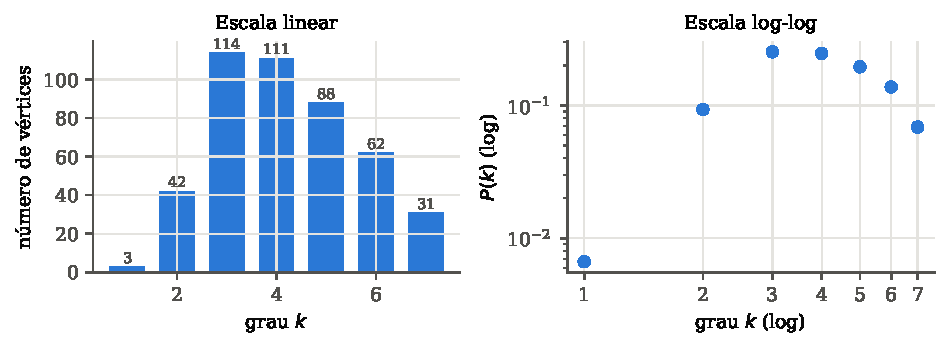
\includegraphics[width=\linewidth]{../figures/distribuicao_graus.pdf}
  \caption{Distribuição de graus em escala linear (esquerda) e log-log (direita).}
  \label{fig:graus}
\end{figure}

\subsection{Parte II: Algoritmos da Disciplina}
Todos os algoritmos foram executados sobre o grafo completo (451 vértices e 951 arestas; 1.241 arcos na versão dirigida). Como o grafo é desconexo, as buscas foram reiniciadas a partir de cada vértice ainda não visitado, cobrindo todas as componentes, e os algoritmos de caminho mínimo de fonte única foram executados a partir de todas as fontes.

\textbf{Busca em largura (BFS).} Implementada com fila (\texttt{deque}), percorre o grafo camada por camada. A varredura completa visitou os 451 vértices em 62 reinícios, confirmando as 62 componentes. Complexidade: $O(V+E)$.

\textbf{Busca em profundidade (DFS).} Implementada com pilha explícita (iterativa). Visitou os 451 vértices. Complexidade: $O(V+E)$.

\textbf{Verificação de Eulerianidade.} Um grafo não-direcionado tem circuito euleriano se é conexo (nas arestas) e todos os vértices têm grau par, e tem caminho euleriano se exatamente dois vértices têm grau ímpar. O grafo completo \textbf{não é euleriano}: é desconexo e possui 236 vértices de grau ímpar. Por partida, 2 componentes admitem circuito euleriano, 15 admitem caminho euleriano e 45 não são eulerianas. Complexidade: $O(V+E)$.

\textbf{Dijkstra.} Implementado com heap binário (\texttt{heapq}) e executado a partir de cada um dos 451 vértices. Encontrou distâncias finitas para os 2.870 pares ordenados intra-partida, isto é, todos os possíveis. A distância média é 2,19 e a máxima é 4,81 (entre \texttt{g05\_p3} e \texttt{g05\_p4}, que quase não se olham). Complexidade: $O((V+E)\log V)$ por fonte.

\textbf{Bellman-Ford.} Executado a partir de cada vértice, com parada antecipada quando uma rodada não relaxa nenhuma aresta. Não encontrou ciclos negativos, o que era esperado, já que $d = -\ln w > 0$. Aqui ele é aplicável, mas desnecessário: Dijkstra é preferível para pesos não-negativos. Complexidade: $O(V \cdot E)$ por fonte.

\textbf{Floyd-Warshall.} Executado no grafo inteiro, gerando uma matriz $451 \times 451$. A implementação ignora $k$ intermediários com $d[i][k] = \infty$, o que, em um grafo particionado em blocos de até 8 vértices, reduz drasticamente o trabalho efetivo. As três abordagens (Dijkstra, Bellman-Ford e Floyd-Warshall) produziram distâncias \textbf{idênticas} para todos os pares. Complexidade: $O(V^3)$.

\textbf{Tarjan.} Implementado na versão iterativa e executado sobre a versão dirigida (1.241 arcos). Encontrou 131 componentes fortemente conexas (SCCs): 62 não-triviais, exatamente uma por partida, e 69 unitárias. Em 19 partidas, todos os participantes formam uma única SCC. As SCCs unitárias revelam assimetria de atenção: 62 participantes (13,7\%) não recebem atenção acima do uniforme de nenhum colega e, portanto, não podem estar em um ciclo dirigido. Complexidade: $O(V+E)$.

\textbf{Prim e Kruskal.} Como o grafo é desconexo, ambos produzem uma \emph{floresta} geradora mínima. Prim é reiniciado em cada componente e usa heap mínimo; Kruskal usa \textit{union-find} com compressão de caminho e união por posto. Ambos encontraram 389 arestas ($V - 62$, uma árvore por partida) com o mesmo peso total, 551,96. A floresta conecta cada partida pelos pares de maior atenção mútua. Complexidade: $O(E\log V)$.

\subsubsection{Resumo dos resultados}
A Tabela~\ref{tab:tempos} e a Figura~\ref{fig:tempos} comparam a complexidade teórica com o tempo observado.

\begin{table*}[t]
  \caption{Complexidade teórica e tempo real observado (em milissegundos), com IC de 95\%. $V = 451$, $E = 951$ (1.241 arcos no Tarjan).}
  \label{tab:tempos}
  \begin{tabular}{llrrrc}
    \toprule
    Algoritmo & Complexidade & $n$ & Média (ms) & Desvio (ms) & IC 95\% (ms) \\
    \midrule
    BFS (varredura completa) & $O(V+E)$ & 50 & 0,252 & 0,247 & [0,184; 0,321] \\
    DFS (varredura completa) & $O(V+E)$ & 50 & 0,369 & 0,144 & [0,329; 0,409] \\
    Eulerianidade & $O(V+E)$ & 50 & 0,094 & 0,242 & [0,027; 0,161] \\
    Dijkstra (todas as fontes) & $O(V(V+E)\log V)$ & 50 & 4,801 & 5,136 & [3,377; 6,225] \\
    Bellman-Ford (todas as fontes) & $O(V^2E)$ & 30 & 512,751 & 255,586 & [421,293; 604,210] \\
    Floyd-Warshall & $O(V^3)$ & 10 & 95,384 & 37,860 & [68,301; 122,468]* \\
    Tarjan & $O(V+E)$ & 50 & 0,921 & 1,130 & [0,608; 1,234] \\
    Prim & $O(E\log V)$ & 50 & 0,698 & 0,548 & [0,546; 0,850] \\
    Kruskal & $O(E\log V)$ & 50 & 1,294 & 0,802 & [1,072; 1,516] \\
    \bottomrule
    \multicolumn{6}{l}{\footnotesize * IC calculado com distribuição t-Student ($n = 10$, 9 graus de liberdade); os demais, com distribuição Normal ($n \geq 30$).}
  \end{tabular}
\end{table*}

\begin{figure}[h]
  \centering
  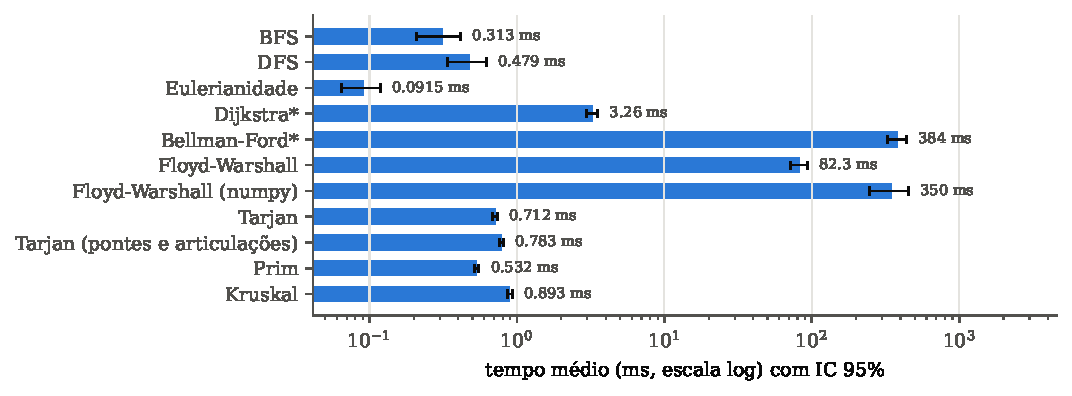
\includegraphics[width=\linewidth]{../figures/tempos.pdf}
  \caption{Tempo médio de cada algoritmo (escala logarítmica) com IC de 95\%. * indica execução a partir de todas as fontes.}
  \label{fig:tempos}
\end{figure}

Os algoritmos lineares ficam abaixo de 1,5 ms. Bellman-Ford a partir de todas as fontes é o mais lento: cada execução percorre os 1.902 arcos da lista global em cada rodada, inclusive arcos de partidas inalcançáveis a partir da fonte. Floyd-Warshall, mesmo sendo $O(V^3) \approx 9{,}2 \times 10^7$ no pior caso, foi 5 vezes mais rápido que Bellman-Ford graças à poda de intermediários inalcançáveis. Os desvios relativamente altos se devem ao ruído do sistema operacional em medições de submilissegundos.

\subsection{Parte III: Análise de Propriedades da Rede}

\subsubsection{Propriedade small-world}
Uma rede é \textit{small-world} quando $L \approx L_{rand}$ e $C \gg C_{rand}$, o que se resume pelo coeficiente $\sigma = (C/C_{rand})/(L/L_{rand})$, com $\sigma > 1$ indicando a propriedade. Implementamos o gerador $G(n,m)$ e comparamos o grafo com dois aleatórios equivalentes, cada um com 30 amostras: (i) o \textbf{global}, com mesmos $n$ e $m$; e (ii) o \textbf{por blocos}, que sorteia, dentro de cada partida, o mesmo número de arestas observado nela.

\begin{table}[h]
  \caption{Comparação com grafos aleatórios equivalentes (média de 30 amostras).}
  \label{tab:sw}
  \begin{adjustbox}{max width=\columnwidth}
  \begin{tabular}{lrrr}
    \toprule
    Métrica & Observado & $G(n,m)$ global & $G(n,m)$ por blocos \\
    \midrule
    Clusterização $C$ & 0,7541 & 0,0080 & 0,6599 \\
    Comprimento médio $L$ & 1,3401 & 4,3851 & 1,3459 \\
    Componentes & 62 & 5,6 & 62 \\
    $C/C_{rand}$ & -- & 94,4 & 1,14 \\
    $L/L_{rand}$ & -- & 0,31 & 1,00 \\
    $\sigma$ & -- & \textbf{309,1} & \textbf{1,15} \\
    \bottomrule
  \end{tabular}
  \end{adjustbox}
\end{table}

Contra o aleatório global, o grafo pareceria fortemente \textit{small-world} ($\sigma = 309$). Essa conclusão, porém, é um artefato: o aleatório global ignora que as interações só podem ocorrer dentro de uma partida. Quando essa restrição é respeitada, $L$ coincide com o aleatório ($1{,}34$ contra $1{,}35$) e a clusterização é apenas 14\% maior ($\sigma = 1{,}15$).

\textbf{Faz sentido para este grafo?} Só parcialmente. Dentro de cada partida, todos estão a no máximo 3 passos, mas isso decorre do tamanho minúsculo dos grupos ($\leq 8$ pessoas), não de atalhos de longo alcance. Entre partidas a distância é infinita, então a rede como um todo não é \textit{small-world}. O pequeno excesso de clusterização ($\sigma = 1{,}15$) indica que o fechamento triádico é um pouco maior do que o acaso explicaria.

\textbf{Implicação prática.} Em uma rede \textit{small-world}, informação e influência se propagam em poucos passos. Aqui, dentro de uma mesa de jogo, qualquer olhar ou sinal pode alcançar todos em um ou dois intermediários, o que favorece a coordenação rápida (e a detecção de comportamentos suspeitos). Por outro lado, nada se propaga entre partidas.

\subsubsection{Lei de potência}
Investigamos se $P(k) \sim k^{-\gamma}$. A Figura~\ref{fig:lp} mostra a distribuição em escala log-log com o ajuste linear e a distribuição de Poisson de mesma média, além da CCDF.

\begin{figure}[h]
  \centering
  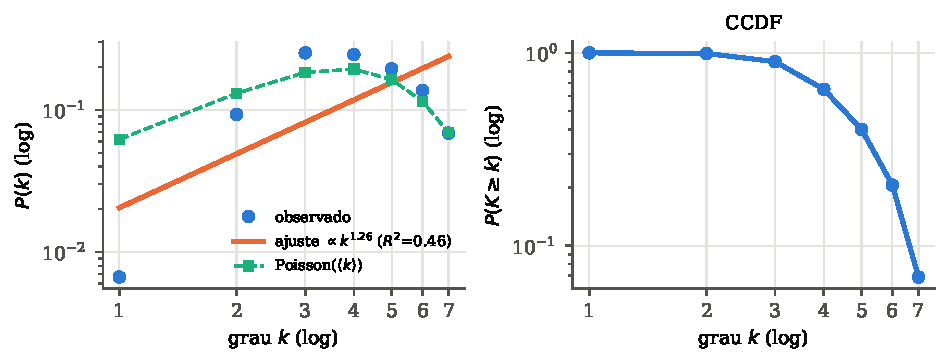
\includegraphics[width=\linewidth]{../figures/lei_potencia.pdf}
  \caption{Distribuição de graus em escala log-log com ajuste de lei de potência e Poisson de mesma média (esquerda) e CCDF (direita).}
  \label{fig:lp}
\end{figure}

\textbf{A distribuição não sugere lei de potência.} A regressão em log-log tem inclinação \emph{positiva} ($P(k) \propto k^{+1{,}26}$) e $R^2 = 0{,}46$: os pontos não formam uma reta decrescente, e sim uma curva com máximo em $k = 3$. A CCDF cai abruptamente após $k = 4$, em vez de decair lentamente. Além disso, a razão $k_{max}/\langle k \rangle = 1{,}66$ indica ausência de hubs, e a variância dos graus ($2{,}00$) é menor que a média ($4{,}22$). A distribuição é \emph{subdispersa} e se aproxima mais de uma Poisson (curva verde) do que de uma lei de potência. Faz sentido: o grau é limitado pelo tamanho da partida ($k \leq 7$), o que impede qualquer cauda pesada.

\subsubsection{Robustez}
Como o grafo é desconexo, a política adotada foi analisar o grafo completo (todas as 62 componentes), já que a LCC tem apenas 8 vértices. Removemos $r = \lfloor 0{,}05 \times 451 \rfloor = 22$ vértices em três cenários: remoção aleatória (30 repetições), ataque por grau e ataque por \textit{betweenness}. Nos ataques, a centralidade foi calculada uma vez (ranking fixo) com implementação própria do algoritmo de Brandes. Medimos: (A) tamanho da LCC e fração de vértices no maior pedaço conexo da própria partida; (B) número de componentes; (C) comprimento médio e eficiência global $E = \frac{1}{n(n-1)}\sum_{u\neq v} 1/d(u,v)$; e (D) fração de vértices isolados.

\begin{table}[h]
  \caption{Métricas de robustez após a remoção de 5\% dos vértices (aleatória: média $\pm$ desvio de 30 repetições).}
  \label{tab:rob}
  \begin{adjustbox}{max width=\columnwidth}
  \begin{tabular}{lrrrr}
    \toprule
    Métrica & Original & Aleatória & Grau & Betw. \\
    \midrule
    A: LCC & 8 & 8 $\pm$ 0 & 8 & 8 \\
    A: fração no núcleo & 1,000 & 0,951 $\pm$ 0,001 & 0,945 & 0,933 \\
    B: componentes & 62 & 62,1 $\pm$ 0,3 & 65 & 68 \\
    C: comprimento médio & 1,340 & 1,342 $\pm$ 0,006 & 1,395 & 1,394 \\
    C: eficiência ($\times 10^{-2}$) & 1,175 & 1,177 $\pm$ 0,01 & 1,126 & 1,118 \\
    D: isolados (\%) & 0,00 & 0,03 $\pm$ 0,08 & 0,70 & 1,17 \\
    \bottomrule
  \end{tabular}
  \end{adjustbox}
\end{table}

\begin{figure}[h]
  \centering
  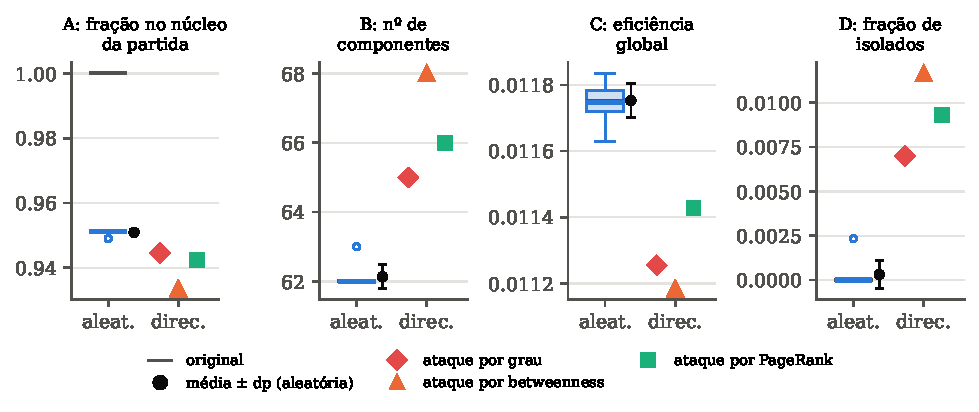
\includegraphics[width=\linewidth]{../figures/robustez.pdf}
  \caption{Remoção aleatória (boxplot de 30 repetições, com média $\pm$ desvio) contra ataques direcionados por grau (losango) e \textit{betweenness} (triângulo).}
  \label{fig:rob}
\end{figure}

\textbf{Remoção aleatória: robusta.} A fração no núcleo cai para 0,951, praticamente o limite trivial $1 - 22/451 = 0{,}951$: os vértices removidos saem, mas quase nenhum sobrevivente é desconectado. O número de componentes fica estável ($62{,}1$), e o comprimento médio e a eficiência não se alteram.

\textbf{Ataque direcionado: também robusta.} O ataque degrada a rede mais que o acaso (até 68 componentes e 1,2\% de isolados com \textit{betweenness}), mas a diferença é pequena: a fração no núcleo cai apenas de 0,951 para 0,933. Não há um colapso como o observado em redes livres de escala. Como $k_{max} = 7$ e a clusterização é alta, não existem hubs cuja remoção fragmente a rede, e cada partida tem caminhos redundantes. Além disso, os 22 vértices mais centrais estão espalhados por 17 (grau) e 20 (\textit{betweenness}) partidas distintas, de modo que o ataque é diluído entre componentes independentes. A \textit{betweenness} foi ligeiramente mais eficaz que o grau por mirar justamente os poucos vértices-ponte dentro das partidas.

\subsubsection{Descoberta mais interessante}
A descoberta mais interessante foi que \textbf{toda a estrutura global do grafo é explicada pela partição em partidas}. Um modelo nulo que conhece apenas quantas arestas há em cada partida reproduz quase exatamente o comprimento médio ($L$: 1,34 contra 1,35), o número de componentes e 88\% da clusterização. O valor $\sigma = 309$, que sugeriria uma rede \textit{small-world} exemplar, é um artefato da escolha do modelo nulo. Isso ilustra um cuidado metodológico importante: o grafo aleatório de referência precisa respeitar as restrições físicas do sistema (aqui, quem pode olhar para quem).

A estrutura \emph{fina} está na direção das arestas: apenas 46,7\% dos arcos são recíprocos, 62 participantes (13,7\%) não recebem atenção acima do uniforme de ninguém, e o participante mais olhado de cada partida recebe em média 30\% dos arcos. Ou seja, a atenção em um jogo de dedução social é assimétrica e concentrada, justamente o tipo de padrão que os autores do dataset exploram para detectar enganadores~\cite{kumar2021}.

\subsubsection{Extra: aproximação a modelos clássicos}
Geramos, com implementações próprias, grafos Erdős–Rényi ($G(n,m)$), Barabási–Albert ($m_0 = 2$) e Watts–Strogatz ($k = 4$, $p = 0{,}1$) com $n = 451$ e número de arestas próximo de 951 (média de 10 amostras).

\begin{table}[h]
  \caption{Comparação com modelos clássicos (média de 10 amostras).}
  \label{tab:modelos}
  \begin{adjustbox}{max width=\columnwidth}
  \begin{tabular}{lrrrrr}
    \toprule
    Modelo & $k_{max}$ & Var($k$) & $C$ & $L$ & Comp. \\
    \midrule
    Observado & 7 & 2,00 & 0,754 & 1,34 & 62 \\
    Erdős–Rényi & 11,7 & 4,01 & 0,009 & 4,40 & 4,0 \\
    Barabási–Albert & 62,0 & 25,42 & 0,065 & 3,69 & 1 \\
    Watts–Strogatz & 6,0 & 0,40 & 0,373 & 7,36 & 1 \\
    \bottomrule
  \end{tabular}
  \end{adjustbox}
\end{table}

Globalmente, \textbf{nenhum dos três modelos descreve o grafo}. Barabási–Albert gera hubs ($k_{max} = 62$) inexistentes aqui. Erdős–Rényi e Watts–Strogatz produzem redes conexas com caminhos longos e clusterização baixa ou moderada. Localmente, contudo, cada partida se aproxima de um \textbf{Erdős–Rényi denso} $G(n, p)$ com $p \approx 0{,}67$: o modelo por blocos reproduz $L$ e quase toda a clusterização (Tabela~\ref{tab:sw}). O modelo que melhor descreve a rede inteira é, portanto, a união disjunta de grafos aleatórios densos, um caso extremo de modelo de blocos estocástico sem arestas entre blocos.

\section{Discussão Crítica}
A análise revelou uma rede muito diferente das redes de grande escala tipicamente estudadas, e a comparação ajuda a entender o alcance de cada conceito.

\textbf{Escala e exatidão.} Por ter apenas 451 vértices, o grafo permitiu calcular todas as métricas de forma exata, executar Floyd-Warshall no grafo completo e validar Dijkstra, Bellman-Ford e Floyd-Warshall entre si em todos os 2.870 pares. Em compensação, as medições de tempo ficaram na faixa de submilissegundos, onde o ruído do sistema domina e inflaciona o desvio padrão.

\textbf{Sensibilidade ao tratamento.} A topologia depende fortemente do limiar. Sem limiar, o grafo seria a união de 62 cliques quase completas ($C \approx 1$, diâmetro 1), e quase toda análise seria trivial. O limiar $1/N$ é interpretável, mas outros critérios (por exemplo, $f \geq 0{,}10$ ou apenas arestas recíprocas) mudariam densidade e clusterização. Uma extensão natural seria repetir as análises para vários limiares e avaliar a estabilidade das conclusões.

\textbf{Perda de informação temporal.} A agregação em um grafo estático descarta a dinâmica da conversa: quem olha para quem enquanto alguém fala, mudanças de foco ao longo das rodadas e o comportamento dos espiões em momentos-chave. Os papéis dos jogadores (espião ou não) também não estão disponíveis nos arquivos de rede, o que impediu relacionar a assimetria de atenção à enganação.

\textbf{Conceitos dependentes do modelo nulo.} O caso do \textit{small-world} mostra que métricas comparativas só são informativas quando o modelo nulo é adequado. O mesmo vale para a robustez: a métrica clássica ``tamanho da LCC'' é inútil aqui (vale 8 em todos os cenários), o que motivou a métrica complementar de fração no núcleo da partida.

\textbf{Desempenho dos algoritmos.} Os algoritmos $O(V+E)$ (BFS, DFS, Eulerianidade e Tarjan) foram os mais rápidos, como esperado. Kruskal foi mais lento que Prim pelo custo da ordenação global das arestas. A observação mais didática é que a estrutura do grafo altera a ordem prática dos algoritmos: Floyd-Warshall, de pior complexidade assintótica, superou Bellman-Ford a partir de todas as fontes, porque a poda de intermediários inalcançáveis explora a partição em blocos.

\section{Conclusão}
Este trabalho analisou o grafo G16 (\textit{comm-f2f-Resistance}) do SNAP, determinado pela matrícula 224215945. A partir de 3,1 milhões de arestas temporais, um pipeline de tratamento (agregação temporal, remoção do laptop, limiar de atenção, simetrização e união das partidas) produziu um grafo de 451 vértices, 951 arestas e 62 componentes. As principais conclusões são:

\begin{itemize}
  \item A rede é a união de 62 grupos densos (densidade intra-partida de 0,67), com clusterização alta ($0{,}75$), diâmetro máximo 3 e grau limitado a 7;
  \item Há indícios aparentes de \textit{small-world} contra um aleatório global ($\sigma = 309$), mas eles desaparecem com um modelo nulo que respeita as partidas ($\sigma = 1{,}15$); os caminhos curtos resultam do tamanho dos grupos;
  \item A distribuição de graus \textbf{não} segue lei de potência: é subdispersa, sem hubs e próxima de uma Poisson;
  \item A rede é robusta tanto a falhas aleatórias quanto a ataques direcionados, por não possuir hubs e por ter alta redundância local;
  \item Todos os algoritmos da disciplina foram aplicados ao grafo completo, com resultados validados entre si e contra uma biblioteca de referência;
  \item A informação mais rica está na direção das arestas: a atenção é assimétrica (46,7\% de reciprocidade) e concentrada em poucos participantes por partida.
\end{itemize}

\begin{thebibliography}{9}
\bibitem{kumar2021} KUMAR, Srijan; BAI, Chongyang; SUBRAHMANIAN, V. S.; LESKOVEC, Jure. Deception Detection in Group Video Conversations using Dynamic Interaction Networks. In: \textit{International AAAI Conference on Web and Social Media (ICWSM)}, 2021.
\bibitem{bai2019} BAI, Chongyang et al. Predicting the Visual Focus of Attention in Multi-Person Discussion Videos. In: \textit{International Joint Conference on Artificial Intelligence (IJCAI)}, 2019.
\bibitem{snap} LESKOVEC, Jure; KREVL, Andrej. \textit{SNAP Datasets: Stanford Large Network Dataset Collection}, 2014. Disponível em: \url{https://snap.stanford.edu/data}.
\bibitem{cormen} CORMEN, Thomas H. et al. \textit{Introduction to Algorithms}. 4. ed. Cambridge: MIT Press, 2022.
\bibitem{barabasi} BARABÁSI, Albert-László. \textit{Network Science}. Cambridge: Cambridge University Press, 2016. Disponível em: \url{http://networksciencebook.com}.
\bibitem{watts} WATTS, Duncan J.; STROGATZ, Steven H. Collective dynamics of `small-world' networks. \textit{Nature}, v. 393, p. 440--442, 1998.
\end{thebibliography}

\end{document}
